\begin{figure}
	\centering
	\begin{tabular}{c|ccc}
		Predictor & \multicolumn{3}{c}{Extractor} \\
		\midrule
		& \iter{} & \gridex{} & \cart{} \\
		\subfloat[LR.]{
			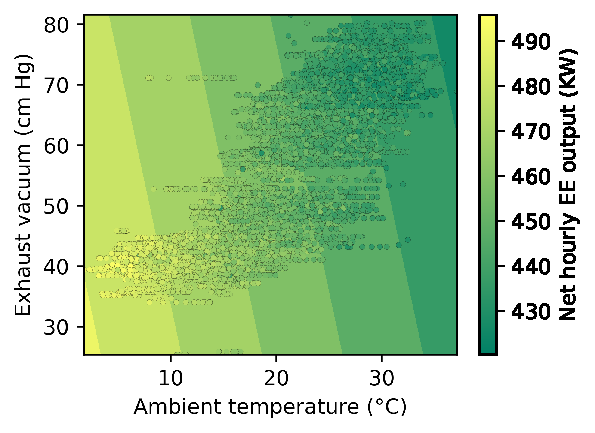
\includegraphics[width=0.215\linewidth]{figures/REG/bb-lr.pdf}
			\label{fig:bb-lr}
		} &
		\subfloat[]{
			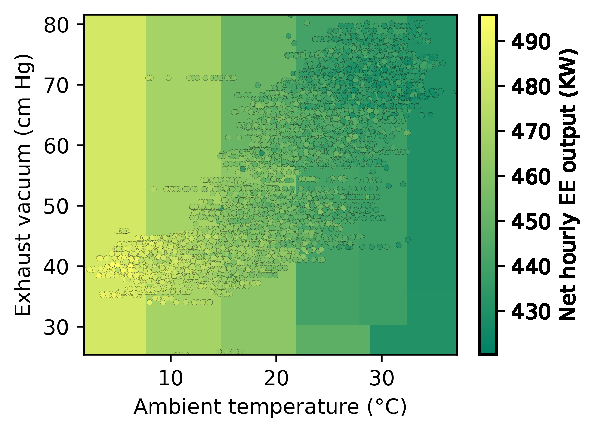
\includegraphics[width=0.2\linewidth]{figures/REG/iter-lr.pdf}
			\label{fig:iter-lr}
		} &
		\subfloat[]{
			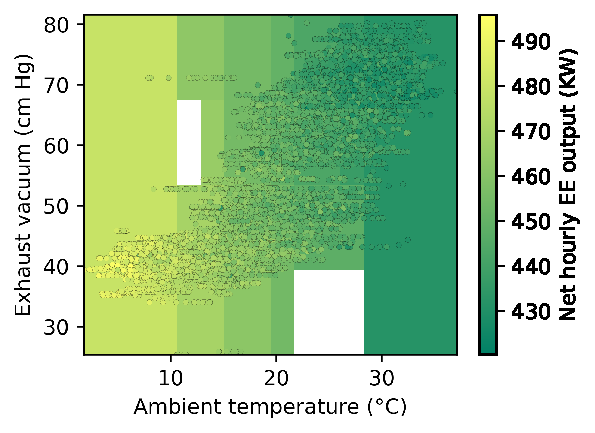
\includegraphics[width=0.2\linewidth]{figures/REG/gridex-lr.pdf}
			\label{fig:gridex-lr}
		} &
		\subfloat[]{
			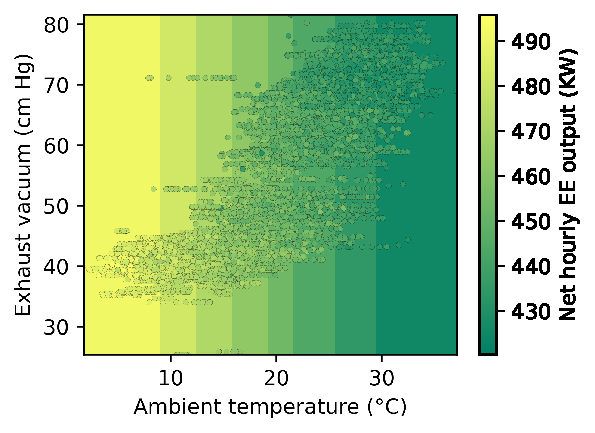
\includegraphics[width=0.2\linewidth]{figures/REG/cart-lr.pdf}
			\label{fig:cart-lr}
		} \\
		%&
		\subfloat[MLP.]{
			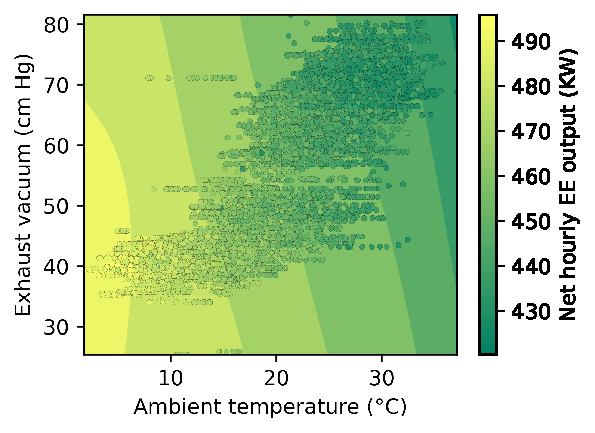
\includegraphics[width=0.2\linewidth]{figures/REG/bb-mlp.pdf}
			\label{fig:bb-mlp}
		} &
		\subfloat[]{
			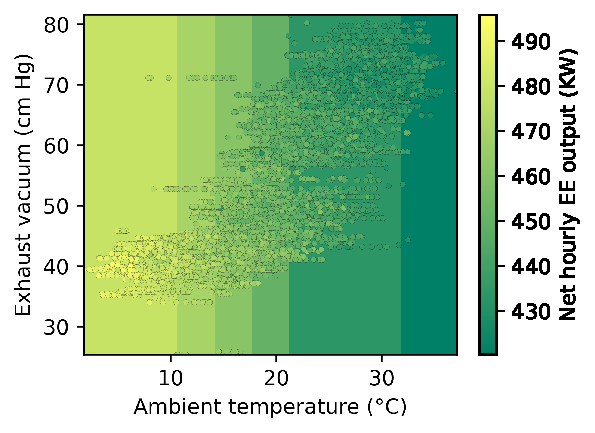
\includegraphics[width=0.2\linewidth]{figures/REG/iter-mlp.pdf}
			\label{fig:iter-mlp}
		} &
		\subfloat[]{
			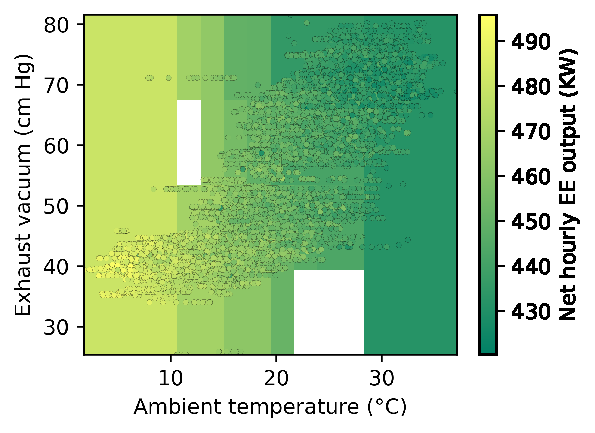
\includegraphics[width=0.2\linewidth]{figures/REG/gridex-mlp.pdf}
			\label{fig:gridex-mlp}
		} &
		\subfloat[]{
			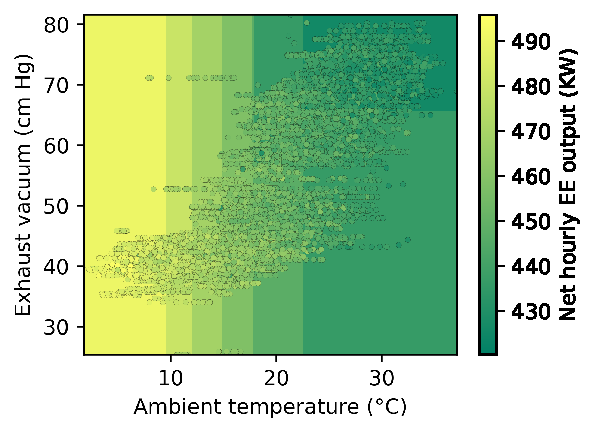
\includegraphics[width=0.2\linewidth]{figures/REG/cart-mlp.pdf}
			\label{fig:cart-mlp}
		} \\		
		%&		
		\subfloat[DT.]{
			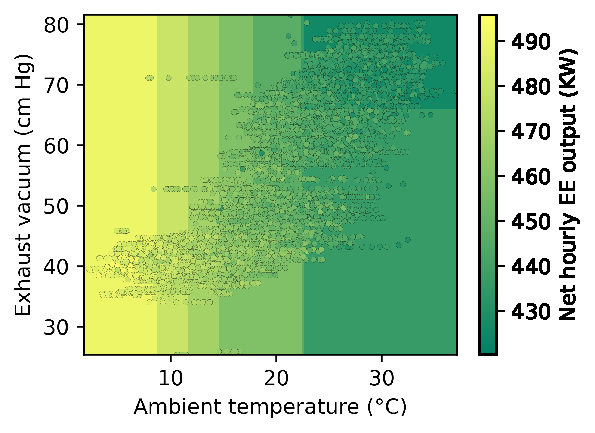
\includegraphics[width=0.2\linewidth]{figures/REG/bb-dt.pdf}
			\label{fig:bb-dt}
		} &
		\subfloat[]{
			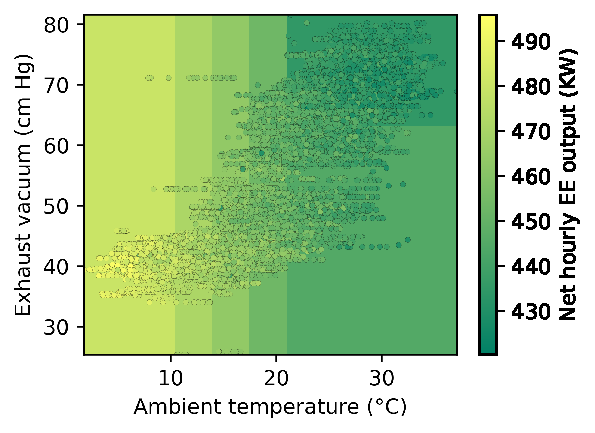
\includegraphics[width=0.2\linewidth]{figures/REG/iter-dt.pdf}
			\label{fig:iter-dt}
		} &
		\subfloat[]{
			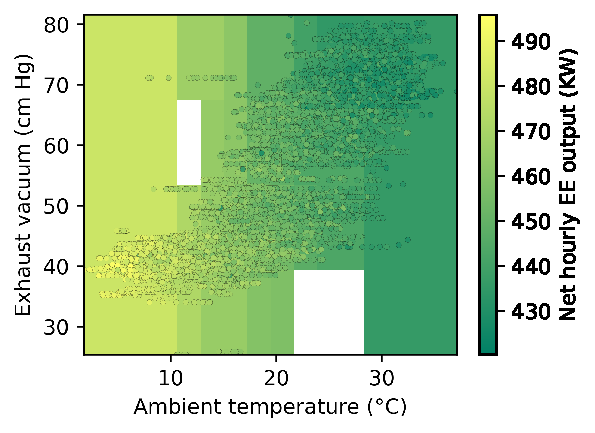
\includegraphics[width=0.2\linewidth]{figures/REG/gridex-dt.pdf}
			\label{fig:gridex-dt}
		} &
		\subfloat[]{
			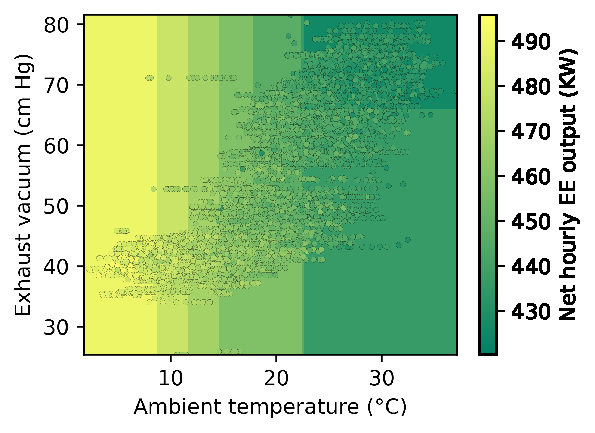
\includegraphics[width=0.2\linewidth]{figures/REG/cart-dt.pdf}
			\label{fig:cart-dt}
		}\\
	\end{tabular}

	\caption{Comparison between CCPP data set output predictions provided by the algorithms implemented in \psyke{}. Only the two most relevant features are reported---i.e., ambient temperature and exhaust vacuum.}
	\label{fig:ccppAll}
\end{figure}